\chapter{Korrelation von Signalen}

\section{Kreuzkorrelationsfunktion}

In der Signalanalyse beschreibt die Kreuzkorrelationsfunktion (KKF) die Korrelation zweier Signale $x(t)$ und $y(t)$ bezüglich einer Zeitverschiebung.\\

Deterministisch \textit{kontinuierlich}
\begin{equation}
\delta{xy}(t) = \int_{-\infty}^{\infty} x(t') y(t'+t) dt
\end{equation}
{\small Mitunter hat die Korrelation ein anderes Vorzeichen, d.h. $t'+t \equiv t'+t$}\\\\

Deterministisch \textit{diskret}
\begin{equation}
R_{xy}(j) = \sum_i x_i y_{i+j}
\end{equation}

Die Normierte Kreuzkorrelationsfunktion
\begin{equation}
R_{xy}(t) = \frac{1}{T_x} \int_{-\infty}^{\infty} x(t') y(t'+t) dt
\end{equation}
{\small Wobei $T_x$ die Länge des Signals $x(t)$ ist.}


\section{Autokorrelationsfunktion}
Die Autokorrelationsfunktion (AKF) bestimmt die Korrelation eines Signals mit sich selbst. Die Korrelation wird analog zur Kreuzkorrelation gebildet.

\subsection{AKF eines stochastischen Prozesses}
Betrachten wir die Autokorrelations als einen stochastischen Prozess in dem der Erwartungswert, $E$, des Signals $x(t)$ angenommen werden kann als
\begin{align*}
E[x^2(t)] & < \infty,\\
E[x(t)] & = 0.
\end{align*}
Dann sind die Erwartungswerte der Autokorrelation des Signals $x(t)$
\[
R_{xx}(t) = E[x(t_1)\,x(t_2)].
\]
Liegt eine schwache Stationalität des gemessenen Signals vor ist die Autokorrelation
\[
R_{xx}(t_1, t_2) = R_{xx}(t+t_1, t+t_2)
\]
{\small $\forall\,t, t_1, t_2$}\\\\
Die \textit{Autokovarianzfunktion} ist so nur vom Timelag $\tau = t_2 - t_1$ abhängig,
\[
R_{xx}(t_1, t_1+\tau) = R_{xx}(\tau) = E[x(t), x(t+\tau)].
\]
Das führt zur zu folgendem Ausdruck der Autokorrelationsfunktion:
\begin{equation}
R_{xx}(\tau) = \frac{R_{xx}(\tau)}{R_{xx}(0)}
\end{equation}


\subsection{Schätzung der AKF}
Die Schätzung der Autokorrelationsfunktion mithilfe von diskreten Realisierungen kann geschrieben werden als Normierte Summe
\[
\hat R_{xx}(i) = \frac{1}{N-i} \sum_{j=0}^{N-i} x_j\,x_{j+i}
\]
Die \textit{erwartungstreue} Schätzung der Korrelation
\[
E[\hat R_{xx}(i)] = \frac{1}{N-i} \sum_{j=0}^{N-i} E[x_j,\,x_{j+i}]
\]

\section{Korrelation und Faltung}
Vergleicht man die Faltung mit Korrelationsfunktion zeigen sich folgende Identitäten
\[
F\{x(t) \ast y(t)\} = x(\omega)\,y(\omega) = |X(\omega)| |Y(\omega)|\,e^{\varphi_x(\omega) + \varphi_y(\omega)},
\]
dies führt zu
\[
F\{R_{xy}\} = x(\omega)\,y^*(\omega) = |X(\omega)| |Y(\omega)|\,e^{\varphi_x(\omega) - \varphi_y(\omega)}.
\]
Man beachte den Vorzeichenwechsel des Phasenantherms.

\subsection*{Faltung der geraden AKF}
Die Faltung der geraden Autokorrelationsfuntion. Wir nehemen an, dass
\[
R_{xx}(t) = R_{xx}(-t).
\]
Dies führt zu zu folgender Identität
\[
F\{R_{xx}(t)\} = |X(\omega)|^2 \Rightarrow \textrm{Powerspektrum}.
\]

\section{Beispiele für Korrelationen}

\subsubsection*{AKF eines Boxcars}
Die Autokorrelation einer Boxcarfunktion.
\begin{figure}[h!]
\centering
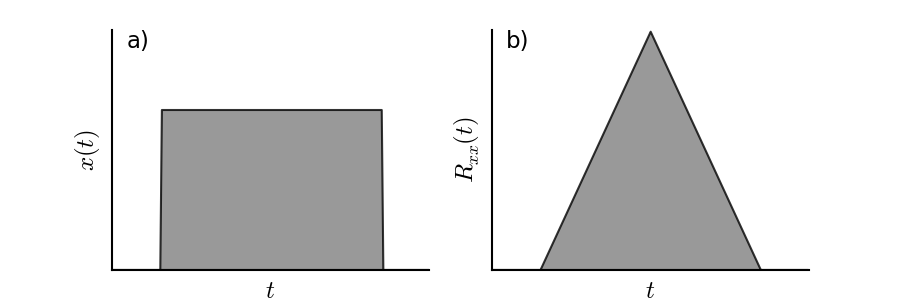
\includegraphics[width=.9\tw]{fig/07-Korrelation/01-example_boxcar.png}
\caption{Schematisches Beispiel der Boxcarfunktion (a) und Autokorrelation derselbigen Boxcarfunktion (b).}
\end{figure}
\begin{align*}
R_{xx}(t) & = \int_{-\infty}^\infty x(t') x(t'+t) dt' \\
& = \begin{cases}
 \int_t^T dt' & -T \leq t \leq 0\\
 \int_0^{T-t} dt' & 0  \leq t \leq T\
 \end{cases}
\end{align*}


\subsubsection*{AKF einer Deltafunktion}
Die Autokorrelationsfunktion einer Deltafunktion, $x(t) = \delta(t)$
\begin{align*}
R_{xx}(t) & = \int_{-\infty}^\infty \delta(t') \delta(t'+t) dt'\\
& = \sigma(t)
\end{align*}

\subsubsection*{Überlagerte Deltafunktionen}
Überlagerung zweier Deltafunktionen mit Amplitude $\delta(t_1) = a$ und $\delta(t_0) = b$ führt zu
\[
R_{xx}(t) = (a^2 + b^2)\delta(t) + ab(\delta(t-t_0) + \delta(t+t_0)).
\]

\begin{figure}[h!]
\centering
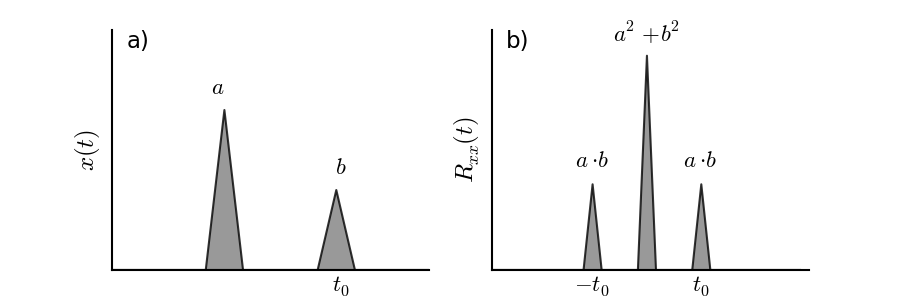
\includegraphics[width=.9\tw]{fig/07-Korrelation/02-example_deltafct.png}
\caption{Schematisches Beispiel zweier Deltafunktionen (a) und Autokorrelation derselbigen Deltafunktpeaks (b).}
\end{figure}

\subsubsection*{AKF bei Nullzahliger Verschiebung}
Die AKF einer Funktion bei $t=0$ folgt:
\[
R_{xx}(0) = \int_{-\infty}^\infty \delta(t')\,\delta(t') dt' = \int_{-\infty}^\infty \delta(t')^2 dt'.
\]


\subsubsection*{AKF einer harmonischen Schwingung}
Betrachten wir die Schwingung
\[
x(t) = \sin(\omega_0 t)
\]
und die Autokorrelation dieser harmonischen Funktion:
\[
R_xx(t) = \frac{1}{T} \int_{-\infty}^\infty x(t') x(t'+t) dt'
\]
\begin{figure}[h!]
\centering
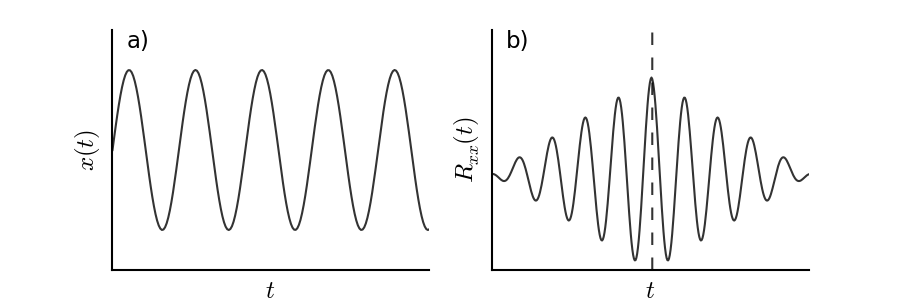
\includegraphics[width=.9\tw]{fig/07-Korrelation/03-example_harmonic.png}
\caption{Schematisches Beispiel einer harmonischen Schwingung (a) und Autokorrelation (b).}
\end{figure}

\subsubsection*{AKF Gaußsche Glockenkurve}
Autokorrelation einer Gaußschen Glockenkurve der Form
\[
x(t) = a\,e^{-t^2/2T^2},
\]
führt zu
\[
R_{xx}(t) = a^2 T \sqrt{\pi} e^{-t^2/4T^2}.
\]

\subsubsection*{AKF eines Sweeps}
Autokorrelation eines Sweeps der Form
\[
\mbox{sweep}(t)=
\begin{cases}
\sin \left(2\pi \left(v_1 + \frac{v_1-v_2}{T} t \right)\right) & t \leq T\\
0& sonst
\end{cases}
\]
Abbildung \ref{fig:korr_sweep} zeigt einen schematischen Sweep und dessen Autokorrelation

\begin{figure}[h!]
\centering
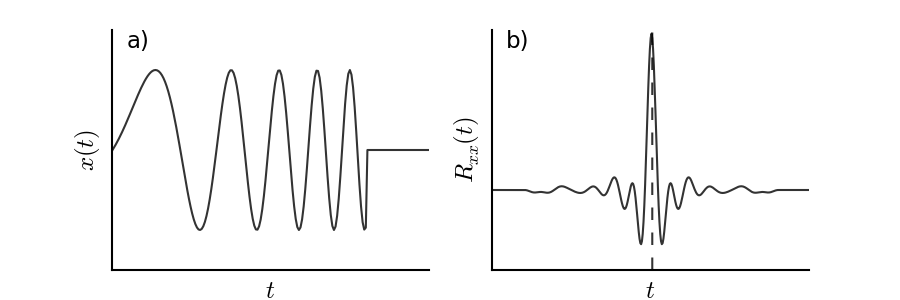
\includegraphics[width=.9\tw]{fig/07-Korrelation/04-example_sweep.png}
\caption{Schematisches Beispiel einer Sweep Funktion (a) und dessen Autokorrelation (b).}
\label{fig:korr_sweep}
\end{figure}

\subsubsection*{AKF von Weißem Rauschen}
Die Autokorrelation von weißem Rauschen,
\[
\{u_i\} = \mbox{iid}.
\]
{\small iid: Independent and identically distributed}\\\\
So folgt die AKF für weißes Rauschen:
\[
R_{uu}(i) = E[u_j + u_{j+i} =
\begin{cases}
\sigma u^2 & i=0\\
0 & \mbox{sonst}
\end{cases}
\]
{\small $\sigma$ ist die Varianz der Amplitude des weißen Rauschens}

\subsubsection*{AKF von farbigem Rauschen}
Farbiges Rauschen ist gleichverteiltes Rauschen in einem begrenzten Frequenzband.
\[
F\{R_{xx}(i)\} = \mbox{const.} = |N(\omega)|^2
\]

\subsubsection*{AKF einer Seismischen Spur}
{\color{red}Formeln müssen überarbeitet werden!}\\\\
Die Autokorrelation einer Seismischen Spur $s$ kann betrachtet werden als
\[
s_i = w_i * x_i.
\]
{\small Dabei ist $w_i$ das Wavelet und $x_i$ die Reflektivität.}
$x_i$ ist gleichverteilt:
\begin{align*}
\{x_i\} = \mbox{iid ZP} & & R_{xx}(i) = \sigma x^2 \, \sigma(\hat{t})^2
\end{align*}
{\small iid ZP: unabhängiger Zufallsprozess}\\
Dann ist der Erwartungswert der Autokorrelation des Signals:
\begin{align*}
R_{ss}(i) & = E[s_j\, s_{j+i}]\\
& = E\left[\sum_k w_k, x_{j-k}\, \sum_l w_l x_{j+i-l}\right]\\
& = \sum_k \sum_l w_l\,E[x_{j-k}\,x_{j+i-l}]\\
& \not= 0
\begin{cases}
Nur & j-k = j+i-l\\
Oder & l = i+k
\end{cases}
\end{align*}
Daraus folt, dass die Autokorrelation der Seismischen Spur etwa der Autokorrelation des Wavelets entspricht:
\[
R_{ss}(i) \sim R_{ww}(i) = \sigma x^2 \, \sum_k w_k \, w_{k+1} < \sigma x^2 R_{ww}(i)
\]
So kann der Frequenzgehalt des initialen Wavelets aus der Seismischen Spur oder Seismogramm abgelesen werden.

\subsubsection*{AKF Seismische Spur mit Ghost}
Autokorrelation einer Seismischen Spur mit dem Ghost der Reflektion. Anwedung in der Prozessierung von reflektionsseismischen Daten.
\[
y_i = s_i * g_i.
\]
{\small Wobei $g_i$ der Ghostoperator ist}\\\\
Im Frequenzbereich:
\[
Y(\omega) = S(\omega) \cdot G(\omega)
\]
So ist die Fouriertransformierte der Autokorrelation
\begin{align*}
F\{R_{yy}(i)\}\;Y(\omega)\,Y*(\omega) & = S(\omega) G(\omega) S*(\omega) G*(\omega)\\
& = F\{R_{gg}\},
\end{align*}
was uns zu
\[
R_{yy}(i) = R_{ss}(i)*R_{gg}(i)
\]
führt.

\section{Ambient Noise - Greensche Funktionen aus Rauschen}
Die Greensche Funktion zwischen zwei Seismometer Stationen kann durch wiederholte Korrelation und Stapelung aus dem Hintergrundrauschen (\textit{Ambient Noise}) bestimmt werden. Dafür ist eine lange Registrierung des Rauschens an den zwei Stationen notwendig, Tage, Monate oder Jahre.

\subsection{Datenbearbeitung}
\subsubsection*{Vorbereitende Datenbearbeitung}
Ist man allein an dem Hintergrundrauschen interessiert sind Erbebensignale Störsignale und müssen aus der Signalreihe gefiltert werden.\\
Dazu kann die Zeitreihe z.B. mit der inversen der Envelope (siehe Sektion \ref{sec:signalyse_envelope}) gewichten werden, so werden die Signale mit hohen Energien im Zeitbereich gering Gewichtet.

\subsubsection*{Korrelation}
Korrelation der einzelnen Segmente (z.B. 12 oder 24 Stunden Segmente)
\[
R_{s_1 s_2}(t)
\]

\subsubsection*{Whitening im Frequenzbereich}
Um alle Signale gleich zu betrachten wird ein \textit{whitening} der Kreuzkorrelation im Frequenzbereich durchgeführt. Das heisst dass die Amplituden aller Frquenzen im Signal 1 ist. Starke Frequenzen werden herunter gewichtet und schwache hoch.

\subsubsection*{Rücktransformation und Stapelung}
Nach anschließender Rücktransformation in den Zeitbereich werden die Kreuzkorrelationen aller Segmente gestapelt um die Greensche Funktion zwischen dem Stationspaar zu erhalten.